\section{Problem statement}
\label{bi-axial-shear-mohr-coulomb:sec:problem-statement}

Inspired by the Plaxis 3D Validation Manual a bi-axial shear test of a
homogenous material block of $\SI{1}{\metre} \times \SI{1}{\metre} \times
    \SI{1}{\metre}$ should be modeled to test the limit load resulting from the
Mohr-Coulomb failure criterion. The test setup is shown in
\autoref{bi-axial-shear-mohr-coulomb:fig:setup}. At xmin, ymin, ymax, and zmin
the block is fixed perpendicular to the face. The face xmax is loaded with a
constant (normal) pressure of $\sigma'_2 =
    \qty{1}{\kilo\newton\per\square\metre}$. The (normal) pressure $\sigma'_1$ at
zmax ramps up till no convergence can be found anymore. Material parameters are
given in \autoref{bi-axial-shear-mohr-coulomb:material-parameters}.

\begin{table}[htbp]
    \centering
    \caption{Material parameters}
    \label{bi-axial-shear-mohr-coulomb:material-parameters}
    \begin{tabularx}{\textwidth}{XYY}

        \hline

        Property                        & Physical unit                                         & Value       \\

        \hline

        Youngs modulus $E$              & \si[per-mode = symbol]{\kilo\newton\per\square\metre} &
        \SI{1000}{}                                                                                           \\

        Poisson's ratio $\nu$           & -                                                     & \SI{0.25}{} \\

        Angle of inner friction $\phi'$ & \si[per-mode = symbol]{\degree}                       & \SI{30}{}
        \\

        Cohesion $c'$                   & \si[per-mode = symbol]{\kilo\newton\per\square\metre} & 1           \\

        \hline
    \end{tabularx}
\end{table}

\begin{figure}[htbp]
    \centering
    \begin{tikzpicture}

        % this image has been generated using Blender writing a SVG
        % using the "Freestyle SVG Exporter". The SVG is minimized
        % using third-party tools and finally converted to PDF using
        % Inkscape.
        \node[inner sep=0pt] (ch-stresses) at (0,0) {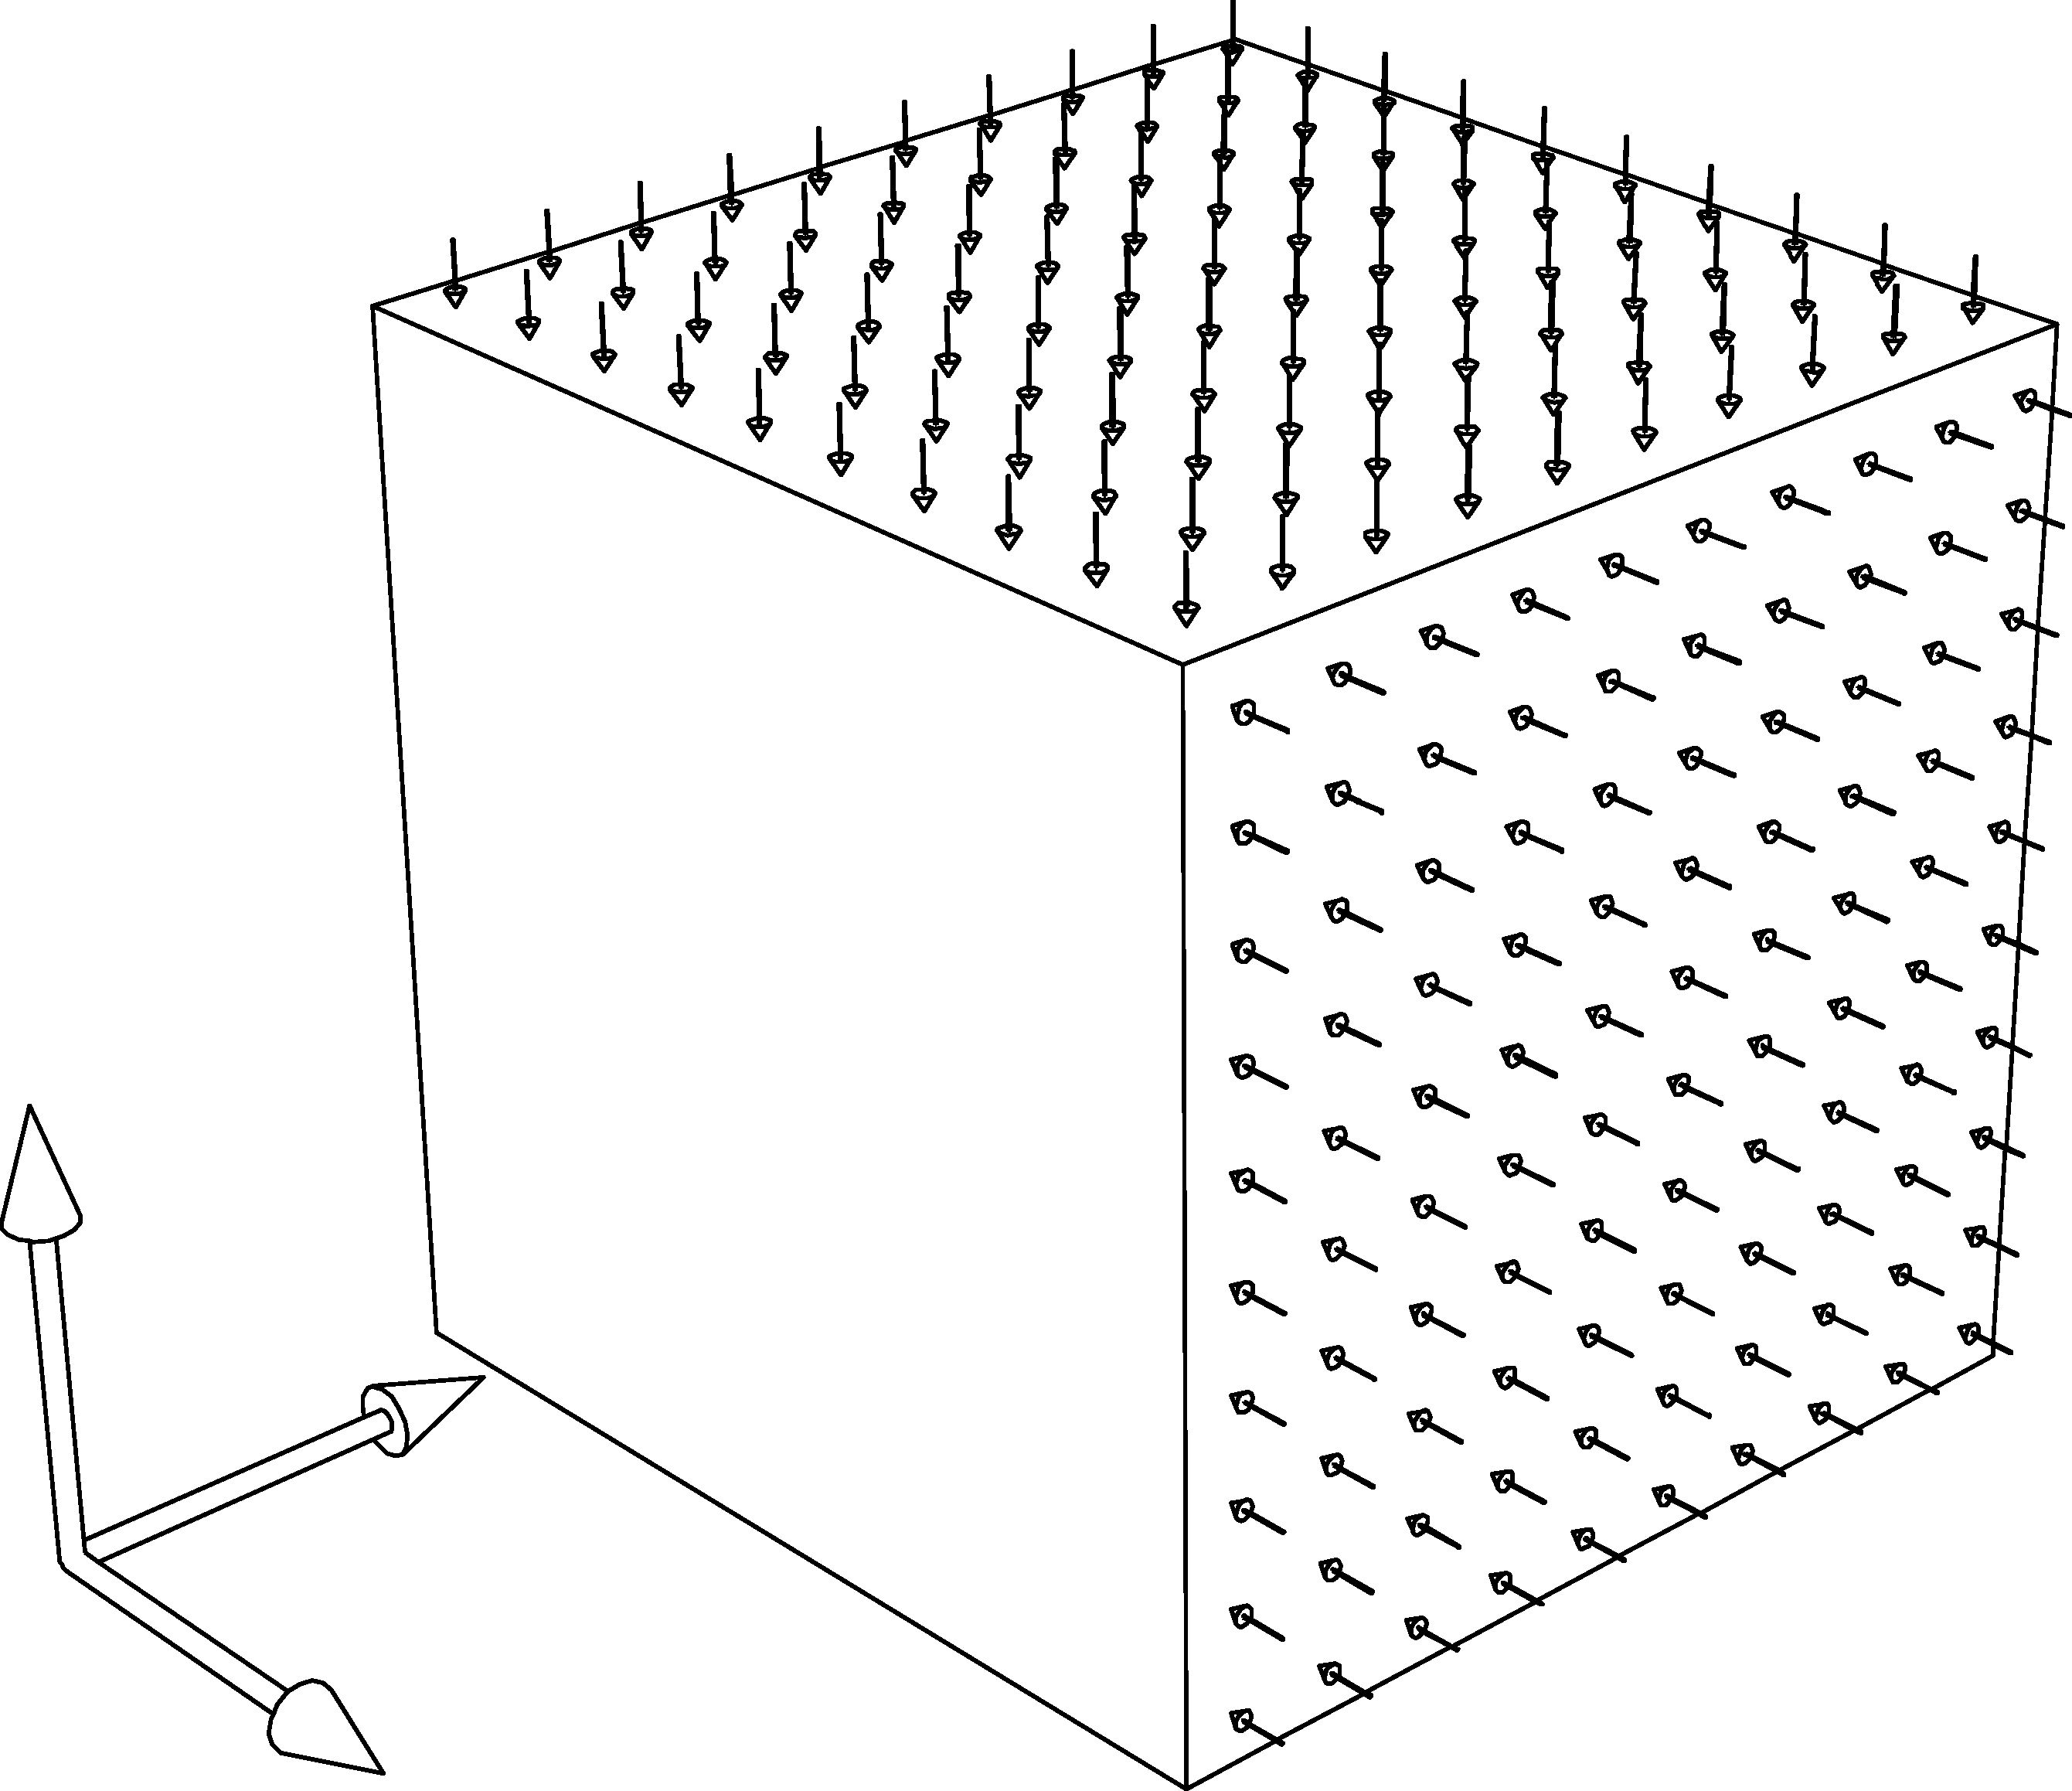
\includegraphics[width=0.4\linewidth]{\currfiledir/bi-axial-shear.blend.svg.pdf}};

        \node[] at (-3.0,-2.9) {x};
        \node[] at (-2.5,-1.5) {y};
        \node[] at (-3.0,-1.0) {z};

        \node[draw,circle,fill=white,minimum size=.5cm,inner sep=0pt, text width=1.5cm, align=center] (xmin_text) at (-3.5,+2.7) {xmin: $u_x \equiv 0$};
        \node (xmin) at (-2.1,+1.0) {};
        \path[->] (xmin_text) edge [out=270, in=160] (xmin);

        \node[draw,circle,fill=white,minimum size=.5cm,inner sep=0pt, text width=2.0cm, align=center] (xmax_text) at (+4.5,-2.5) {xmax: \\ $\sigma'_2 \equiv \qty[per-mode = fraction]{1}{\kilo\newton\per\square\metre} $};
        \node (xmax) at (+2.2,-1.4) {};
        \path[->] (xmax_text) edge [out=180, in=0] (xmax);

        \node[draw,circle,fill=white,minimum size=.5cm,inner sep=0pt, text width=1.5cm, align=center] (ymin_text) at (-3.8,+0.3) {ymin: $u_y \equiv 0$};
        \node (ymin) at (-0.8,-0.7) {};
        \path[->] (ymin_text) edge [out=0, in=180] (ymin);

        \node[draw,circle,fill=white,minimum size=.5cm,inner sep=0pt, text width=1.5cm, align=center] (ymax_text) at (+4.8,+1.7) {ymax: $u_y \equiv 0$};
        \node (ymax) at (+3.3,+0.0) {};
        \path[->] (ymax_text) edge [out=270, in=20] (ymax);

        \node[draw,circle,fill=white,minimum size=.5cm,inner sep=0pt, text width=1.5cm, align=center] (zmin_text) at (-1.2,-3.5) {zmin: $u_z \equiv 0$};
        \node (zmin) at (+0.2,-2.8) {};
        \path[->] (zmin_text) edge [out=0, in=270] (zmin);

        \node[draw,circle,fill=white,minimum size=.5cm,inner sep=0pt, text width=1.2cm, align=center] (zmax_text) at (+2.4,+3.2) {zmax: $\sigma'_1 = ?$};
        \node (zmax) at (+0.4,+1.7) {};
        \path[->] (zmax_text) edge [out=180, in=90] (zmax);

    \end{tikzpicture}
    \caption{Setup of the bi-axial shear test}
    \label{bi-axial-shear-mohr-coulomb:fig:setup}
\end{figure}

\section{Analytical solution}
\label{bi-axial-shear-mohr-coulomb:sec:analytical-solution}

From the yield function of the Mohr-Coulomb failure criterion shown in
\autoref{eqn:Mohr-Coulomb-failure-criterion} the limit load of the bi-axial
test can be derived as given in \autoref{eqn:bi-axial-test-limit-load}.

\begin{equation}
    \label{eqn:Mohr-Coulomb-failure-criterion}
    f = \frac{\abs{\sigma'_1 - \sigma'_2}}{2} + \frac{\sigma'_1 + \sigma'_2}{2} \cdot \sin{\phi'} - c' \cdot \cos{\phi'} = 0
\end{equation}

\begin{equation}
    \label{eqn:bi-axial-test-limit-load}
    \sigma'_1 = \sigma'_2 \cdot \frac{1 + \sin{\phi'}}{1 - \sin{\phi'}} - 2c' \cdot \frac{\cos{\phi'}}{1 - \sin{\phi'}}
    \approx \qty{-6.464}{\kilo\newton\per\square\metre}
\end{equation}

\section{Numerical solution with Moose}
\label{bi-axial-shear-mohr-coulomb:sec:moose}

In the corresponding Moose model of this quasi-static problem a discretisation
of \qty{5184}{} TET10 elements and a transient executioner is used. The
linear-elastic material behaviour is modelled with a materials block of type of
\codeword{ComputeIsotropicElasticityTensor}. The ideal-plastic behaviour is
introduced with a materials block of type
\codeword{CappedMohrCoulombStressUpdate}. To avoid the cap of this materials
block to influence the system response, a very high tensile and compressive
strength is used.

The load $\sigma'_1$ ramps up linearly with time so that at $t =
    \qty{6.464}{\second}$ the load is $\sigma'_1 =
    \qty{-6.464}{\kilo\newton\per\square\metre}$. Due to the ideal-plastic nature
of the material behaviour, Moose will attempt to calculate time steps and
iteratively reduce the time step if convergence is not achieved. Eventually the
last converged time step should be at $t \approx \qty{6.464}{\second}$.

This model was calculated using the ‘PJFNK’ solver. The time step is initially
chosen to be \qty{0.25}{\second} and the minimum time step is limited to
\qty{0.001}{\second}. Due to the automatic cut-back of the time steps close to
failure, the last converged time step is at $t=\qty{6.43945}{\second}$. A plot
of the vertical displacement of the box upper face over $\sigma'_1$ can be
found in \autoref{bi-axial-shear-mohr-coulomb:fig:moose-results}. The Moose
input file for this model is attached to this document by the name of
‘bi-axial-shear.i’.

\fileattachment{\currfiledir/bi-axial-shear.i}{bi-axial-shear.i}

\begin{figure}[htbp]
    \centering
    \begin{tikzpicture}
        \begin{axis}[
                xlabel={load on the box top surface $\sigma'_1 (\qty{}{\kilo\newton\per\square\metre})$},
                ylabel style={align=center}, ylabel={vertical displacement of the \\box top surface $u_z$ (\qty{}{\metre})}
            ]
            \addplot
            coordinates {
                    (1,	0)
                    (1.25,	-0.00090138)
                    (1.50,	-0.0011182)
                    (1.75,	-0.0013421)
                    (2.00,	-0.0015701)
                    (2.25,	-0.0018007)
                    (2.50,	-0.002033)
                    (2.75,	-0.0022665)
                    (3.00,	-0.0025008)
                    (3.25,	-0.0027358)
                    (3.50,	-0.0029713)
                    (3.75,	-0.0032072)
                    (4.00,	-0.0034434)
                    (4.25,	-0.0036799)
                    (4.50,	-0.0039166)
                    (4.75,	-0.0041535)
                    (5.00,	-0.0043906)
                    (5.25,	-0.0046279)
                    (5.50,	-0.0048653)
                    (5.75,	-0.0051028)
                    (6.00,	-0.0053404)
                    (6.25,	-0.0055781)
                    (6.375,	-0.005697)
                    (6.4375, -0.0057564)
                    (6.4395, -0.0057583)
                };
            \addplot[mark=*] coordinates {(6.4395, -0.0057783)} node[pin={179, pin distance = 1cm, align=right}:{$\sigma'_1 = \qty[per-mode = symbol]{6.4395}{\kilo\newton\per\square\metre}$\\$u_z \approx \qty{-5.76}{\milli\metre}$}]{} ;
        \end{axis}
    \end{tikzpicture}
    \caption{Vertical displacements of the box top surface in Moose}
    \label{bi-axial-shear-mohr-coulomb:fig:moose-results}
\end{figure}

% arc-length method:
% https://github.com/idaholab/moose/discussions/29932

\section{Numerical solution with Plaxis 3D}
\label{bi-axial-shear-mohr-coulomb:sec:plaxis}

The original model of the bi-axial test as described by Plaxis can be found in
\href{https://bentleysystems.service-now.com/community?id=kb\_article\_view&sysparm_article=KB0110017}{KB0110017}
(PDF via
\href{https://web.archive.org/web/20230926091632/https://communities.bentley.com/cfs-file/\_\_key/communityserver-wikis-components-files/00-00-00-05-58/PlxValidation\_2D00\_Bi\_2D00\_axial\_5F00\_compression\_5F00\_test\_5F00\_with\_5F00\_Mohr\_2D00\_Coulomb\_5F00\_model\_2D00\_2018.pdf}{archive.org}).
In this section an own Plaxis model is used, also following the test setup
described in \autoref{bi-axial-shear-mohr-coulomb:sec:problem-statement}. As
far as possible, the Plaxis default settings have been used unaltered
(including a tolerated error of \qty{0.01}{}).

Main difference to the Moose model is that in Plaxis the calculation type
‘Plastic’ in connection with ‘arc-length control’ is used. While this resembled
not a transient model, it allows Plaxis to follow the unstable load path for
this quasi-static problem.

The discretisation used for Plaxis3D consists of 3093 TET10 elements.

With this model, Plaxis is able to load the block till
\qty{-6.556}{\kilo\newton\per\square\metre} and then reducing the load to
\qty{-6.464}{\kilo\newton\per\square\metre}. This ideal-plastic part of the
system response can be reproduced by the model through the ‘arc-length control’
option. A plot of the vertical displacement of the box upper face over
$\sigma'_1$ can be found in
\autoref{bi-axial-shear-mohr-coulomb:fig:plaxis-results}. The Plaxis command
script file for this model is attached to this document by the name of
‘bi-axial-shear.p3dlog’.

\fileattachment{\currfiledir/bi-axial-shear.p3dlog}{bi-axial-shear.p3dlog}

\begin{figure}[htbp]
    \centering
    \begin{tikzpicture}
        \begin{axis}[
                xlabel={load on the box top surface $\sigma'_1 (\qty{}{\kilo\newton\per\square\metre})$},
                ylabel style={align=center}, ylabel={vertical displacement of the \\box top surface $u_z$ (\qty{}{\metre})}
            ]
            \addplot
            coordinates {
                    (1.00000000000095, -0.000625000000011057)
                    (1.45000004768372, -0.00104687502607703)
                    (1.89999997615814, -0.00146874994970858)
                    (2.34999990463257, -0.00189062498975545)
                    (2.79999995231628, -0.00231250002980232)
                    (3.25, -0.00273437495343387)
                    (3.70000004768372, -0.00315625010989606)
                    (4.15000009536743, -0.00357812503352761)
                    (4.59999990463257, -0.00400000018998981)
                    (5.05000019073486, -0.00442187488079071)
                    (5.5, -0.0048437500372529)
                    (5.94999980926514, -0.0052656251937151)
                    (6.40000009536743, -0.005687499884516)
                    (6.52661514282227, -0.00608526170253754)
                    (6.55597162246704, -0.00645361421629786)
                    (6.52574062347412, -0.00679799681529403)
                    (6.47952795028686, -0.00713548995554447)
                    (6.44913816452026, -0.00747993402183056)
                    (6.44183492660522, -0.00783433578908443)
                    (6.44937801361084, -0.00819497276097536)
                    (6.46049356460571, -0.00855708308517933)
                    (6.46787881851196, -0.00891765765845776)
                    (6.46970701217651, -0.00927593652158976)
                    (6.46782398223877, -0.00963267404586077)
                    (6.46502208709717, -0.00998902786523104)
                    (6.46316385269165, -0.0103457774966955)
                    (6.46270561218262, -0.0107031119987369)
                    (6.46317481994629, -0.0110608329996467)
                    (6.46387243270874, -0.0114186489954591)
                    (6.46433544158936, -0.0117763662710786)
                    (6.46444988250732, -0.012133939191699)
                    (6.46433305740356, -0.0124914143234491)
                    (6.46415901184082, -0.0128488671034575)
                    (6.46404409408569, -0.0132063440978527)
                    (6.46401596069336, -0.0135638574138284)
                    (6.46404552459717, -0.0139213940128684)
                    (6.46408939361572, -0.014278938062489)
                    (6.46411800384521, -0.0146364746615291)
                    (6.46412563323975, -0.0149940028786659)
                    (6.46411800384521, -0.0153515255078673)
                    (6.46410751342773, -0.0157090462744236)
                    (6.46410036087036, -0.0160665679723024)
                    (6.46409845352173, -0.0164240933954716)
                    (6.46410056210040, -0.0167816191080199)
                };
            \addplot[mark=*] coordinates {(6.55597162246704, -0.00645361421629786)} node[pin={179, pin distance = 1cm, align=right}:{$\sigma'_1 = \qty[per-mode = symbol]{6.5560}{\kilo\newton\per\square\metre}$\\$u_z \approx \qty{-6.45}{\milli\metre}$}]{} ;
                \addplot[mark=*] coordinates {(6.46410056210040, -0.01678161910801990)} node[pin={179, pin distance = 1cm, align=right}:{$\sigma'_1 = \qty[per-mode = symbol]{6.4641}{\kilo\newton\per\square\metre}$\\$u_z \approx \qty{-16.78}{\milli\metre}$}]{} ;
        \end{axis}
    \end{tikzpicture}
    \caption{Vertical displacements of the box top surface in Plaxis 3D}
    \label{bi-axial-shear-mohr-coulomb:fig:plaxis-results}
\end{figure}

\section{Summary}
\label{bi-axial-shear-mohr-coulomb:sec:summary}

The bi-axial shear test modeled in this appendix allows both the verification
of the implementation of the Mohr-Coulomb failure criterion in the respective
simulation software and the investigation of the handling of the numerical
instability when the limit load is reached. Both the model in Moose
(\autoref{bi-axial-shear-mohr-coulomb:sec:moose}) and the model in Plaxis
(\autoref{bi-axial-shear-mohr-coulomb:sec:plaxis}) achieve the limit load known
from the analytical solution
(\autoref{bi-axial-shear-mohr-coulomb:sec:analytical-solution}) with good
accuracy.
